\documentclass[twoside]{book}

% Packages required by doxygen
\usepackage{fixltx2e}
\usepackage{calc}
\usepackage{doxygen}
\usepackage[export]{adjustbox} % also loads graphicx
\usepackage{graphicx}
\usepackage[utf8]{inputenc}
\usepackage{makeidx}
\usepackage{multicol}
\usepackage{multirow}
\PassOptionsToPackage{warn}{textcomp}
\usepackage{textcomp}
\usepackage[nointegrals]{wasysym}
\usepackage[table]{xcolor}

% Font selection
\usepackage[T1]{fontenc}
\usepackage[scaled=.90]{helvet}
\usepackage{courier}
\usepackage{amssymb}
\usepackage{sectsty}
\renewcommand{\familydefault}{\sfdefault}
\allsectionsfont{%
  \fontseries{bc}\selectfont%
  \color{darkgray}%
}
\renewcommand{\DoxyLabelFont}{%
  \fontseries{bc}\selectfont%
  \color{darkgray}%
}
\newcommand{\+}{\discretionary{\mbox{\scriptsize$\hookleftarrow$}}{}{}}

% Page & text layout
\usepackage{geometry}
\geometry{%
  a4paper,%
  top=2.5cm,%
  bottom=2.5cm,%
  left=2.5cm,%
  right=2.5cm%
}
\tolerance=750
\hfuzz=15pt
\hbadness=750
\setlength{\emergencystretch}{15pt}
\setlength{\parindent}{0cm}
\setlength{\parskip}{3ex plus 2ex minus 2ex}
\makeatletter
\renewcommand{\paragraph}{%
  \@startsection{paragraph}{4}{0ex}{-1.0ex}{1.0ex}{%
    \normalfont\normalsize\bfseries\SS@parafont%
  }%
}
\renewcommand{\subparagraph}{%
  \@startsection{subparagraph}{5}{0ex}{-1.0ex}{1.0ex}{%
    \normalfont\normalsize\bfseries\SS@subparafont%
  }%
}
\makeatother

% Headers & footers
\usepackage{fancyhdr}
\pagestyle{fancyplain}
\fancyhead[LE]{\fancyplain{}{\bfseries\thepage}}
\fancyhead[CE]{\fancyplain{}{}}
\fancyhead[RE]{\fancyplain{}{\bfseries\leftmark}}
\fancyhead[LO]{\fancyplain{}{\bfseries\rightmark}}
\fancyhead[CO]{\fancyplain{}{}}
\fancyhead[RO]{\fancyplain{}{\bfseries\thepage}}
\fancyfoot[LE]{\fancyplain{}{}}
\fancyfoot[CE]{\fancyplain{}{}}
\fancyfoot[RE]{\fancyplain{}{\bfseries\scriptsize Generated by Doxygen }}
\fancyfoot[LO]{\fancyplain{}{\bfseries\scriptsize Generated by Doxygen }}
\fancyfoot[CO]{\fancyplain{}{}}
\fancyfoot[RO]{\fancyplain{}{}}
\renewcommand{\footrulewidth}{0.4pt}
\renewcommand{\chaptermark}[1]{%
  \markboth{#1}{}%
}
\renewcommand{\sectionmark}[1]{%
  \markright{\thesection\ #1}%
}

% Indices & bibliography
\usepackage{natbib}
\usepackage[titles]{tocloft}
\setcounter{tocdepth}{3}
\setcounter{secnumdepth}{5}
\makeindex

% Hyperlinks (required, but should be loaded last)
\usepackage{ifpdf}
\ifpdf
  \usepackage[pdftex,pagebackref=true]{hyperref}
\else
  \usepackage[ps2pdf,pagebackref=true]{hyperref}
\fi
\hypersetup{%
  colorlinks=true,%
  linkcolor=blue,%
  citecolor=blue,%
  unicode%
}

% Custom commands
\newcommand{\clearemptydoublepage}{%
  \newpage{\pagestyle{empty}\cleardoublepage}%
}

\usepackage{caption}
\captionsetup{labelsep=space,justification=centering,font={bf},singlelinecheck=off,skip=4pt,position=top}

%===== C O N T E N T S =====

\begin{document}

% Titlepage & ToC
\hypersetup{pageanchor=false,
             bookmarksnumbered=true,
             pdfencoding=unicode
            }
\pagenumbering{alph}
\begin{titlepage}
\vspace*{7cm}
\begin{center}%
{\Large as2-\/project-\/\+Frac7 }\\
\vspace*{1cm}
{\large Generated by Doxygen 1.8.13}\\
\end{center}
\end{titlepage}
\clearemptydoublepage
\pagenumbering{roman}
\tableofcontents
\clearemptydoublepage
\pagenumbering{arabic}
\hypersetup{pageanchor=true}

%--- Begin generated contents ---
\chapter{Hierarchical Index}
\section{Class Hierarchy}
This inheritance list is sorted roughly, but not completely, alphabetically\+:\begin{DoxyCompactList}
\item Drawable\+Object\begin{DoxyCompactList}
\item \contentsline{section}{Drawable\+Triangle}{\pageref{classDrawableTriangle}}{}
\item \contentsline{section}{Drawable\+Triangulation}{\pageref{classDrawableTriangulation}}{}
\item \contentsline{section}{Drawable\+Voronoi}{\pageref{classDrawableVoronoi}}{}
\end{DoxyCompactList}
\item Triangle\begin{DoxyCompactList}
\item \contentsline{section}{Drawable\+Triangle}{\pageref{classDrawableTriangle}}{}
\end{DoxyCompactList}
\end{DoxyCompactList}

\chapter{Class Index}
\section{Class List}
Here are the classes, structs, unions and interfaces with brief descriptions\+:\begin{DoxyCompactList}
\item\contentsline{section}{\hyperlink{classDAG}{D\+AG} \\*\hyperlink{classDAG}{D\+AG}\+: search data structure }{\pageref{classDAG}}{}
\item\contentsline{section}{\hyperlink{classNode}{Node} \\*\hyperlink{classNode}{Node}\+: node of the \hyperlink{classDAG}{D\+AG} }{\pageref{classNode}}{}
\item\contentsline{section}{\hyperlink{classTriangle}{Triangle} \\*\hyperlink{classTriangle}{Triangle} }{\pageref{classTriangle}}{}
\item\contentsline{section}{\hyperlink{classTriangulation}{Triangulation} \\*\hyperlink{classTriangulation}{Triangulation}\+: triangles and adjacencies }{\pageref{classTriangulation}}{}
\end{DoxyCompactList}

\chapter{Class Documentation}
\hypertarget{classDrawableTriangle}{}\section{Drawable\+Triangle Class Reference}
\label{classDrawableTriangle}\index{Drawable\+Triangle@{Drawable\+Triangle}}


\hyperlink{classDrawableTriangle}{Drawable\+Triangle}.  




{\ttfamily \#include $<$drawabletriangle.\+h$>$}



Inheritance diagram for Drawable\+Triangle\+:

\hypertarget{classDrawableTriangulation}{}\section{Drawable\+Triangulation Class Reference}
\label{classDrawableTriangulation}\index{Drawable\+Triangulation@{Drawable\+Triangulation}}


\hyperlink{classDrawableTriangulation}{Drawable\+Triangulation}\+: drawable object for the triangulation.  




{\ttfamily \#include $<$drawabletriangulation.\+h$>$}



Inheritance diagram for Drawable\+Triangulation\+:\nopagebreak
\begin{figure}[H]
\begin{center}
\leavevmode
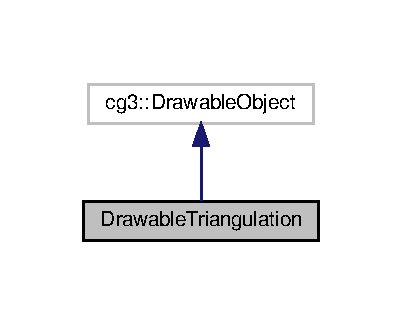
\includegraphics[width=193pt]{classDrawableTriangulation__inherit__graph}
\end{center}
\end{figure}


Collaboration diagram for Drawable\+Triangulation\+:\nopagebreak
\begin{figure}[H]
\begin{center}
\leavevmode
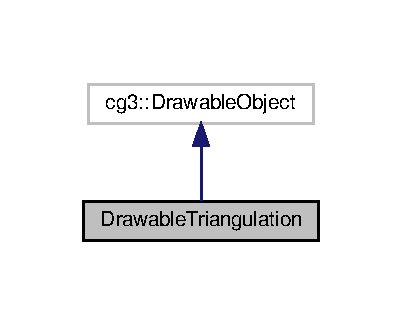
\includegraphics[width=193pt]{classDrawableTriangulation__coll__graph}
\end{center}
\end{figure}
\subsection*{Public Member Functions}
\begin{DoxyCompactItemize}
\item 
\hyperlink{classDrawableTriangulation_a7285109cc73a2d0a233cccd0cb9278a4}{Drawable\+Triangulation} (\hyperlink{classTriangulation}{Triangulation} \&triangulation, \hyperlink{classDAG}{D\+AG} \&dag, const cg3\+::\+Pointd \&center, double radius)
\begin{DoxyCompactList}\small\item\em Initializes the drawable object. \end{DoxyCompactList}\item 
void \hyperlink{classDrawableTriangulation_a364e9b612571481930770fdfa9d68148}{draw} () const
\begin{DoxyCompactList}\small\item\em Draws the triangulation. \end{DoxyCompactList}\item 
cg3\+::\+Pointd \hyperlink{classDrawableTriangulation_a3198ae77285c354fd020f5b18df718f5}{scene\+Center} () const
\begin{DoxyCompactList}\small\item\em Returns the triangulation center. \end{DoxyCompactList}\item 
double \hyperlink{classDrawableTriangulation_a0aee9121b146c327dbbd741c3dc58c0a}{scene\+Radius} () const
\begin{DoxyCompactList}\small\item\em Return the radius of the triangulation. \end{DoxyCompactList}\end{DoxyCompactItemize}


\subsection{Detailed Description}
\hyperlink{classDrawableTriangulation}{Drawable\+Triangulation}\+: drawable object for the triangulation. 

This class inherits only from Drawable\+Object, this implementation follows the composition pattern\+: the drawable object for the triangulation has two members that are references to the \hyperlink{classDAG}{D\+AG}, used to draw only leaves, and to the triangulation data structure. Triangles are drawn using points and lines. 

\subsection{Constructor \& Destructor Documentation}
\mbox{\Hypertarget{classDrawableTriangulation_a7285109cc73a2d0a233cccd0cb9278a4}\label{classDrawableTriangulation_a7285109cc73a2d0a233cccd0cb9278a4}} 
\index{Drawable\+Triangulation@{Drawable\+Triangulation}!Drawable\+Triangulation@{Drawable\+Triangulation}}
\index{Drawable\+Triangulation@{Drawable\+Triangulation}!Drawable\+Triangulation@{Drawable\+Triangulation}}
\subsubsection{\texorpdfstring{Drawable\+Triangulation()}{DrawableTriangulation()}}
{\footnotesize\ttfamily Drawable\+Triangulation\+::\+Drawable\+Triangulation (\begin{DoxyParamCaption}\item[{\hyperlink{classTriangulation}{Triangulation} \&}]{triangulation,  }\item[{\hyperlink{classDAG}{D\+AG} \&}]{dag,  }\item[{const cg3\+::\+Pointd \&}]{center,  }\item[{double}]{radius }\end{DoxyParamCaption})}



Initializes the drawable object. 


\begin{DoxyParams}[1]{Parameters}
\mbox{\tt in}  & {\em triangulation} & array of triangles and adjacencies \\
\hline
\mbox{\tt in}  & {\em dag} & the search data structure \\
\hline
\mbox{\tt in}  & {\em center} & the center of the triangulation -\/ center of the bounding triangle \\
\hline
\mbox{\tt in}  & {\em radius} & the radius of the triangulation -\/ radius of the bounding triangle \\
\hline
\end{DoxyParams}


\subsection{Member Function Documentation}
\mbox{\Hypertarget{classDrawableTriangulation_a364e9b612571481930770fdfa9d68148}\label{classDrawableTriangulation_a364e9b612571481930770fdfa9d68148}} 
\index{Drawable\+Triangulation@{Drawable\+Triangulation}!draw@{draw}}
\index{draw@{draw}!Drawable\+Triangulation@{Drawable\+Triangulation}}
\subsubsection{\texorpdfstring{draw()}{draw()}}
{\footnotesize\ttfamily void Drawable\+Triangulation\+::draw (\begin{DoxyParamCaption}{ }\end{DoxyParamCaption}) const}



Draws the triangulation. 

This method draws only triangles contained in leaves, it draws green lines for the edges and red points for the vertices. \mbox{\Hypertarget{classDrawableTriangulation_a3198ae77285c354fd020f5b18df718f5}\label{classDrawableTriangulation_a3198ae77285c354fd020f5b18df718f5}} 
\index{Drawable\+Triangulation@{Drawable\+Triangulation}!scene\+Center@{scene\+Center}}
\index{scene\+Center@{scene\+Center}!Drawable\+Triangulation@{Drawable\+Triangulation}}
\subsubsection{\texorpdfstring{scene\+Center()}{sceneCenter()}}
{\footnotesize\ttfamily cg3\+::\+Pointd Drawable\+Triangulation\+::scene\+Center (\begin{DoxyParamCaption}{ }\end{DoxyParamCaption}) const}



Returns the triangulation center. 

\begin{DoxyReturn}{Returns}
center\+: the bounding triangle barycenter 
\end{DoxyReturn}
\mbox{\Hypertarget{classDrawableTriangulation_a0aee9121b146c327dbbd741c3dc58c0a}\label{classDrawableTriangulation_a0aee9121b146c327dbbd741c3dc58c0a}} 
\index{Drawable\+Triangulation@{Drawable\+Triangulation}!scene\+Radius@{scene\+Radius}}
\index{scene\+Radius@{scene\+Radius}!Drawable\+Triangulation@{Drawable\+Triangulation}}
\subsubsection{\texorpdfstring{scene\+Radius()}{sceneRadius()}}
{\footnotesize\ttfamily double Drawable\+Triangulation\+::scene\+Radius (\begin{DoxyParamCaption}{ }\end{DoxyParamCaption}) const}



Return the radius of the triangulation. 

\begin{DoxyReturn}{Returns}
radius\+: the bounding triangle radius 
\end{DoxyReturn}


The documentation for this class was generated from the following files\+:\begin{DoxyCompactItemize}
\item 
drawabletriangulation.\+h\item 
drawabletriangulation.\+cpp\end{DoxyCompactItemize}

\hypertarget{classDrawableVoronoi}{}\section{Drawable\+Voronoi Class Reference}
\label{classDrawableVoronoi}\index{Drawable\+Voronoi@{Drawable\+Voronoi}}


\hyperlink{classDrawableVoronoi}{Drawable\+Voronoi}\+: drawable object for Voronoi diagram.  




{\ttfamily \#include $<$drawablevoronoi.\+h$>$}



Inheritance diagram for Drawable\+Voronoi\+:
\nopagebreak
\begin{figure}[H]
\begin{center}
\leavevmode
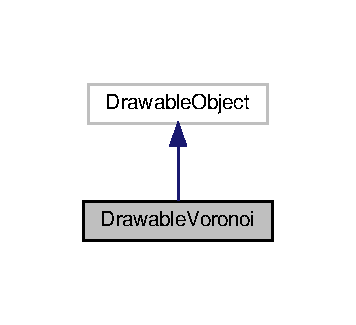
\includegraphics[width=171pt]{classDrawableVoronoi__inherit__graph}
\end{center}
\end{figure}


Collaboration diagram for Drawable\+Voronoi\+:
\nopagebreak
\begin{figure}[H]
\begin{center}
\leavevmode
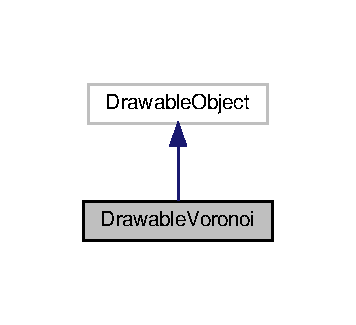
\includegraphics[width=171pt]{classDrawableVoronoi__coll__graph}
\end{center}
\end{figure}
\subsection*{Public Member Functions}
\begin{DoxyCompactItemize}
\item 
\hyperlink{classDrawableVoronoi_aab7fabca89392b0eb45c59b4e695855a}{Drawable\+Voronoi} (\hyperlink{classTriangulation}{Triangulation} \&triangulation, \hyperlink{classDAG}{D\+AG} \&dag, const cg3\+::\+Pointd \&center, const double radius)
\begin{DoxyCompactList}\small\item\em Initializes the drawable object. \end{DoxyCompactList}\item 
void \hyperlink{classDrawableVoronoi_aa10c214cfc42f752433c682760d88b70}{draw} () const
\begin{DoxyCompactList}\small\item\em Draws the Voronoi diagram. \end{DoxyCompactList}\item 
cg3\+::\+Pointd \hyperlink{classDrawableVoronoi_a1707c9e575880eeac9e981d73e03b3bf}{scene\+Center} () const
\begin{DoxyCompactList}\small\item\em Returns the triangulation center. \end{DoxyCompactList}\item 
double \hyperlink{classDrawableVoronoi_af26652a83c96748bf9a09abc6255672b}{scene\+Radius} () const
\begin{DoxyCompactList}\small\item\em Return the radius of the triangulation. \end{DoxyCompactList}\end{DoxyCompactItemize}


\subsection{Detailed Description}
\hyperlink{classDrawableVoronoi}{Drawable\+Voronoi}\+: drawable object for Voronoi diagram. 

This class inherits only from Drawable\+Object, this implementation follows the composition pattern\+: the drawable object for the triangulation has two members that are references to the \hyperlink{classDAG}{D\+AG}, used to draw only leaves, and to the triangulation data structure. The diagram is drawn using circumcenters of each triangle and lines from the circumcenter to the circumcenter of each adjacent triangle. 

\subsection{Constructor \& Destructor Documentation}
\mbox{\Hypertarget{classDrawableVoronoi_aab7fabca89392b0eb45c59b4e695855a}\label{classDrawableVoronoi_aab7fabca89392b0eb45c59b4e695855a}} 
\index{Drawable\+Voronoi@{Drawable\+Voronoi}!Drawable\+Voronoi@{Drawable\+Voronoi}}
\index{Drawable\+Voronoi@{Drawable\+Voronoi}!Drawable\+Voronoi@{Drawable\+Voronoi}}
\subsubsection{\texorpdfstring{Drawable\+Voronoi()}{DrawableVoronoi()}}
{\footnotesize\ttfamily Drawable\+Voronoi\+::\+Drawable\+Voronoi (\begin{DoxyParamCaption}\item[{\hyperlink{classTriangulation}{Triangulation} \&}]{triangulation,  }\item[{\hyperlink{classDAG}{D\+AG} \&}]{dag,  }\item[{const cg3\+::\+Pointd \&}]{center,  }\item[{const double}]{radius }\end{DoxyParamCaption})}



Initializes the drawable object. 


\begin{DoxyParams}[1]{Parameters}
\mbox{\tt in}  & {\em triangulation} & array of triangles and adjacencies \\
\hline
\mbox{\tt in}  & {\em dag} & the search data structure \\
\hline
\mbox{\tt in}  & {\em center} & the center of the triangulation -\/ center of the bounding triangle \\
\hline
\mbox{\tt in}  & {\em radius} & the radius of the triangulation -\/ radius of the bounding triangle \\
\hline
\end{DoxyParams}


\subsection{Member Function Documentation}
\mbox{\Hypertarget{classDrawableVoronoi_aa10c214cfc42f752433c682760d88b70}\label{classDrawableVoronoi_aa10c214cfc42f752433c682760d88b70}} 
\index{Drawable\+Voronoi@{Drawable\+Voronoi}!draw@{draw}}
\index{draw@{draw}!Drawable\+Voronoi@{Drawable\+Voronoi}}
\subsubsection{\texorpdfstring{draw()}{draw()}}
{\footnotesize\ttfamily void Drawable\+Voronoi\+::draw (\begin{DoxyParamCaption}{ }\end{DoxyParamCaption}) const}



Draws the Voronoi diagram. 

This method draws only triangles contained in leaves, it draws blue lines for the edges and yellow points for the circumcenters. \mbox{\Hypertarget{classDrawableVoronoi_a1707c9e575880eeac9e981d73e03b3bf}\label{classDrawableVoronoi_a1707c9e575880eeac9e981d73e03b3bf}} 
\index{Drawable\+Voronoi@{Drawable\+Voronoi}!scene\+Center@{scene\+Center}}
\index{scene\+Center@{scene\+Center}!Drawable\+Voronoi@{Drawable\+Voronoi}}
\subsubsection{\texorpdfstring{scene\+Center()}{sceneCenter()}}
{\footnotesize\ttfamily cg3\+::\+Pointd Drawable\+Voronoi\+::scene\+Center (\begin{DoxyParamCaption}{ }\end{DoxyParamCaption}) const}



Returns the triangulation center. 

\begin{DoxyReturn}{Returns}
center\+: the bounding triangle barycenter 
\end{DoxyReturn}
\mbox{\Hypertarget{classDrawableVoronoi_af26652a83c96748bf9a09abc6255672b}\label{classDrawableVoronoi_af26652a83c96748bf9a09abc6255672b}} 
\index{Drawable\+Voronoi@{Drawable\+Voronoi}!scene\+Radius@{scene\+Radius}}
\index{scene\+Radius@{scene\+Radius}!Drawable\+Voronoi@{Drawable\+Voronoi}}
\subsubsection{\texorpdfstring{scene\+Radius()}{sceneRadius()}}
{\footnotesize\ttfamily double Drawable\+Voronoi\+::scene\+Radius (\begin{DoxyParamCaption}{ }\end{DoxyParamCaption}) const}



Return the radius of the triangulation. 

\begin{DoxyReturn}{Returns}
radius\+: the bounding triangle radius 
\end{DoxyReturn}


The documentation for this class was generated from the following files\+:\begin{DoxyCompactItemize}
\item 
drawablevoronoi.\+h\item 
drawablevoronoi.\+cpp\end{DoxyCompactItemize}

%--- End generated contents ---

% Index
\backmatter
\newpage
\phantomsection
\clearemptydoublepage
\addcontentsline{toc}{chapter}{Index}
\printindex

\end{document}
